\documentclass[a4paper, 10pt]{article}
\usepackage[utf8]{inputenc}
\usepackage[spanish]{babel}
\usepackage{graphicx}
\usepackage{geometry}
\usepackage{listings}
\usepackage{amsmath}
\usepackage{amsfonts}
\usepackage{amssymb}
\usepackage{caratula}
\usepackage[section]{placeins}
\usepackage{titlesec}
\usepackage[colorlinks=true,linkcolor=blue,urlcolor=black,bookmarksopen=true]{hyperref}
\usepackage{bookmark}
\usepackage{float}

\newcommand{\Z}{\mathbb{Z}}
\def\code#1{\texttt{#1}}
\newcommand\tab[1][0.5cm]{\hspace*{#1}}

\geometry{a4paper, margin=0.7in}

\begin{document}
    %Caratula
    \pagenumbering{gobble}
    \newpage

    \begin{center}
        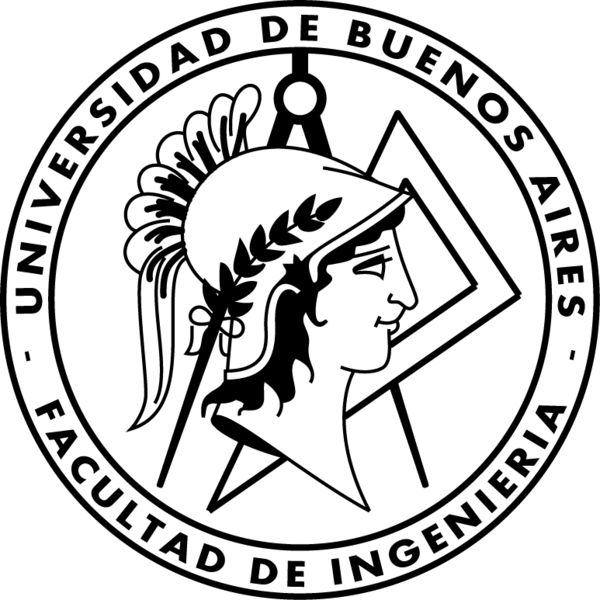
\includegraphics[width=7.5cm, height=7.5cm]{images/logo}
    \end{center}

    \materia{Organización de Datos}
    \submateria{Segundo Cuatrimestre 2017}
    \titulo{Trabajo Práctico 2}

    \integrante{Rodrigo De Rosa}{97799}{rodrigoderosa@outlook.com}
    \integrante{Marcos Schapira}{97934}{schapiramarcos@gmail.com}
    \integrante{Facundo Guerrero}{97981}{facundoiguerrero@gmail.com}
    \maketitle
    %Fin caratula
    %Table of contents
    \newpage
    \pagenumbering{roman}
    \tableofcontents
    %Fin table of contents
    %Informe
    \newpage
	\pagenumbering{arabic}
	\section{Resumen}
	
		Luego de procesar los datos de acuerdo a las conclusiones obtenidas en el primer trabajo, aplicando distintos algoritmos para realizar la predicción, obtuvimos los mejores resultados mediante Gradient Boosting Regressor utilizando:
		\begin{itemize}
		
		\item \emph{División de propiedades en grupos de acuerdo al metro cuadrado}
			
		\item \emph{Superficie total}

		\item \emph{Tipo de propiedad} 
			
		\end{itemize}
		
		Esto nos lleva a pensar que la predicción de precios de propiedades de Properati se puede estimar con certeza hasta cierto punto, ya que los datos están altamente comprometidos con graves inconsistencias tanto en precio como en superficie. Recomendamos a la empresa revisar su proceso de recolección de datos exhaustivamente. 		
		
	\section{Adaptación de los datos}
		
		Antes de lanzarse a la predicción, se deben procesar los datos de una manera consistente (mayormente con el análisis de TP1) para así acercarse lo mas posible a una estimación correcta. Las siguientes son las conclusiones mas fuertes que obtuvimos del primer trabajo.
		
		\subsection{Rango coherente de variación de precio por metro cuadrado}
		Al igual que en el primer trabajo práctico, se recortaron los datos según su precio por metro cuadrado para de esta manera tratar de
		quedarnos con datos que tuvieran el mayor 'sentido' posible. Estos recortes se hicieron superior e inferiormente, de la misma manera
		que en el primer trabajo.
		
		\subsection{División por grupos acorde al precio por metro cuadrado}
		A partir del análisis realizado en el primer trabajo práctico, en el que se dividió a los barrios en seis grupos según su precio por
		metro cuadrado, surgió la idea de codificar a cada barrio a partir de su posición en el ranking de precio por metro cuadrado; es decir,
		se le asignó un número a cada barrio que depende de su precio por metro cuadrado y la distancia de un barrio al próximo depende de que
		tanto mayor es su precio. De esta manera, se buscó determinar una distancia unidimensional entre los barrios que no dependa de su
		ubicación geográfica sino del valor de su suelo.
			
		\subsection{La propiedades con mayores precios dentro de capital se ubican cerca de paradas del subterráneo}
		
		Para esto procesamos la columna de "Cantidad de Paradas de Transporte Publico Cercanas". A grandes rasgos la utilizamos de 2 maneras, primero para los datos completos y segundo separando para CABA y GBA (tanto usándolas o no en GBA). Bajo estos criterios variamos las escalas de los valores y fuimos analizando como se comportaban con los distintos algoritmos probando una gran cantidad de variaciones sin tener mucho éxito.

		\subsection{La cantidad de locales gastronómicos y escuelas dan resultados similares sobre los centros mas importantes} 
		
		Como ya anticipamos en el tp anterior, los locales gastronómicos y las escuelas cercanos nos brindan información similar. Es por esto que probamos tanto utilizando ambas para el calculo como solo una o ninguna. A la vez también variamos las escalas de estas. 
			
		\subsection{La ubicación en general influye en el precio}
		Procesamos las columnas de latitud y longitud tanto unidas como separadas, para tratar de darle una influencia individual a la ubicación.
		
		\subsection{Conclusiones}
		Los mejores resultados sin embargo, los obtuvimos sin tener en cuenta gran parte de las consideraciones recién planteadas, básicamente el único análisis que causo impacto fue el del precio por metro cuadrado. Esto comienza a anticipar la inconsistencia de los datos del set de prueba y como el análisis hecho en el trabajo anterior tiene sentido para datos consistentes con el mundo real. 		
		
		
	\section{Estimación de las superficies faltantes en el set de prueba}
		Ya que los algoritmos de predicción no pueden recibir entradas del tipo "nan" tuvimos que plantear distintas estrategias para solucionar esto. Se completo mediante la mediana general, el promedio general, e incluso sacando un promedio por barrios, sin embargo el mejor resultado se obtuvo mediante llenarlo con el valor de mayor frecuencia.
		
		\subsection{Conclusiones}
		Dentro de este mismo tema notamos algo realmente interesante. Siendo 14166 el total de propiedades en el set a estimar, 120 de estas tienen un tamaño menor a 9 metros cuadrados (tamaño mínimo reglamentario de una celda de prisión), e incluso parte de estas se encuentran en los barrios mas caros de la región a analizar. Esto agrega mayor importancia a la idea de que los datos de prueba no son de muy buena calidad. 
	
	\section{Algoritmos de predicción}
		Todos los algoritmos los analizamos de acuerdo a cross validation cambiando las distintas proporciones entre set de entrenamiento y test. El set de datos para el entrenamiento fue el que utilizamos en el primer trabajo en donde ya están descartadas todas las propiedades que no tienen mucho sentido y dañan al set (mas que nada por superficies y precios por metro cuadrado ilógicos). Esto sin embargo no impide que el set de datos tenga las mismas anomalías. Al tener que calcularlas igual es imposible evitar el gran error de antemano con el que se encuentra este segundo trabajo. Los siguientes fueron los algoritmos que se utilizaron junto con sus mejores combinaciones. Se utilizaran las implementaciones por la librería scikit-learn \footnote{http://scikit$-$learn.org/stable/}. 
		
		\subsection{Random Forest Regressor}
		
			Luego de un análisis previo sobre problemas similares de este tipo, e incluso de competencias de Kaggle internacionales sobre estimación de precios de propiedades, todas coinciden en que este algoritmo es de los mas adecuados para utilizar. Luego de llegar a muy buenos resultados usando las columnas "place value", "superficie", "tipo de propiedad", "cantidad de paradas de transporte", "cantidad de locales gastronómicos", y "latitud y longitud" se obtuvieron realmente buenos resultados con bajos errores de rmse. Sin embargo al subir los resultados a Kaggle estos dan muy lejos de lo calculado. Luego de quitar columnas y dejando el algoritmo mas simple se lograron mejores resultados con solo "place value", "superficie", y "tipo de propiedad". Algo similar ocurrió con el siguiente algoritmo Gradient Boost Regressor. Siendo que este ultimo suele ser particularmente robusto contra overfitting, se sostiene la teoría de que los datos de prueba presentan una cantidad importante de inconsistencias. Los hiperparametros para este mejor caso son:
			 
		\begin{itemize}
		
		\item \emph{n estimators=100}
			
		\item \emph{max features='log2'}

		\item \emph{min samples leaf=2}
		
		\item \emph{min samples split=4}
		
		\item \emph{bootstrap=True}
		
		\item \emph{oob score=True} 
			
		\end{itemize}
		
		\subsection{Gradient Boosting}
			Al igual que con Random Forest, el uso de este algoritmo surge de la investigación; es conocido como 'el algoritmo que nunca anda
			del todo mal' y aquí no fue una excepción. También al igual que en Random Forest, se comenzó utilizando varios features resultantes
			del análisis del TP1 pero finalmente los mejores resultados se obtuvieron con 'place value', 'superficie' y 'tipo de propiedad'. \\
			\tab Luego de realizar algunos Grid Searchs, este algoritmo dio los mejores resultados a partir de los siguientes hiperparámetros:
			\begin{itemize}
				\item \emph{n estimators = 5000}
				\item \emph{learning rate = 0.241}
				\item \emph{max depth = 5} 
			\end{itemize}
			\tab Cabe destacar que se realizaron pruebas tanto con la librería \emph{sklearn} como con la librería \emph{XGBoost} para comparar
			resultados y tratar de obtener el mejor posible. Los mejores resultados se obtuvieron con la primera.
		\subsection{Ada Boost}
		\subsection{Extra Regressor}
		\subsection{KNN}
		\subsection{Ensambles}		
		
		\subsection{Conclusiones}
			El mejor resultado se obtuvo con Gradient Boost Regressor llegando a dar los dentro del mismo orden que los mejores resultados de la competencia.
			
		\section{Conclusiones Generales y Recomendaciones}
		
			Luego de todo el análisis realizado de acuerdo a los resultados obtenidos concluimos que efectivamente el set de datos a predecir esta repleto de anomalías e inconsistencias. Esto genera que una buena predicción implica una cobertura baja de los datos ya que estimar correctamente cuestiones sin sentido solo se logra mediante azar y generar un overfitting sobre el caso de prueba en cuestión.\\
			Sobre la empresa Properati, recomendamos aplicar un análisis sobre la forma en que los datos son cargados a su pagina, incluso teniendo en cuenta la posibilidad de prohibir resultados absurdos (como por ejemplo propiedades de 0 metros de superficie). Siendo que se manejan cuestiones sensibles de mucho dinero, la pagina podría ser vulnerable a casos de corrupción donde terceros puedan aprovechar el sistema para realizar acciones ilícitas. Por ultimo queremos resaltar que nos llama fuertemente la atención la cantidad de propiedades vendidas por mes, siendo un numero, según nuestra consideración, exorbitante.	
			
\end{document}
